\problemname{Extreme Sort}

John likes sorting algorithms very much. He has studied quicksort, merge sort,
radix sort, and many more.

A long time ago he has written a lock-free parallel string sorting program. It
was a combination of burstsort and multi-key quicksort. To implement burstsort
you need to build a tree of buckets. For each input string you walk through the
tree and insert part of the string into the right bucket. When a bucket fills
up, it "bursts" and becomes a new subtree (with new buckets).

\begin{figure}[h]
	\centering
	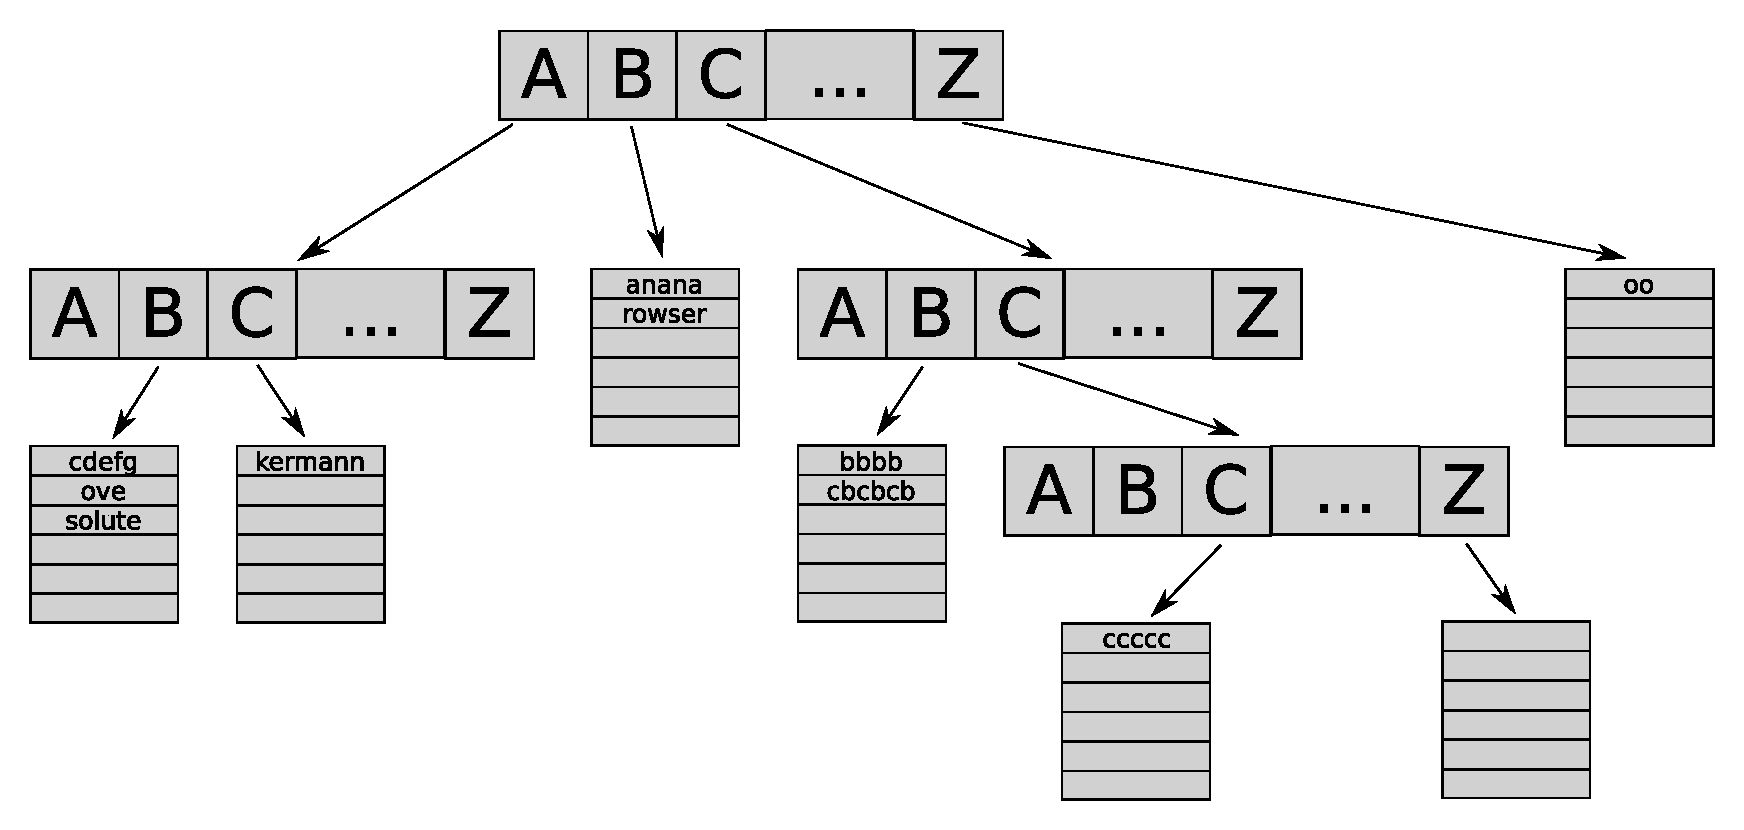
\includegraphics[height=6cm]{burstsort.pdf}
	\caption{Burstsort data structure}
\end{figure}

Well, enough about the past. Today John is playing with sorting algorithms
again. This time it's numbers. He has an idea for a new algorithm, ``extreme
sort''. It's extremely fast, performance levels are OVER NINETHOUSAND. Before
he tells anyone any details, he wants to make sure that it works correctly.

Your task is to help him and verify that the so-called \emph{extreme property} holds after the
first phase of the algorithm.
The extreme property is defined as
$ \min\left( x_{i,j} \right) \geq 0 $, where

\begin{equation*}
    x_{i,j} =
   \begin{cases}
	   a_j - a_i & \text{for} \quad 1 \leq i < j \leq N \\
	   9001      & \text{otherwise}
   \end{cases}
\end{equation*}

\section*{Input}
The first line contains a single integer $N$ ($1 \le N \le 1024$).
The second line contains $N$ integers $a_1 \; a_2 \; \ldots \; a_N$ ($1 \le a_i \le 1024$).

\section*{Output}
Print one line of output containing
``{\tt yes}'' if the extreme property holds for the given input,
``{\tt no}'' otherwise.
